Tomando el diseño conceptual como base y ya teniendo un modelo de clasificación
con un poder impresionante para distinguir entre las células atípicas. Podemos
convertir el sistema, aislado y desconectado de su aplicación final, y
transmutarlo en una solución final para el problema de diagnóstico de
\hyperlink{abbr}{CCU} mediante análisis citológico. En la
\autoref{fig:despliegue} podemos ver que este proceso de despliegue recibe un
sistema y, aplicando técnicas de ingeniería de software, lo convertimos en una
solución final.

\begin{figure}[H]
    \centering
    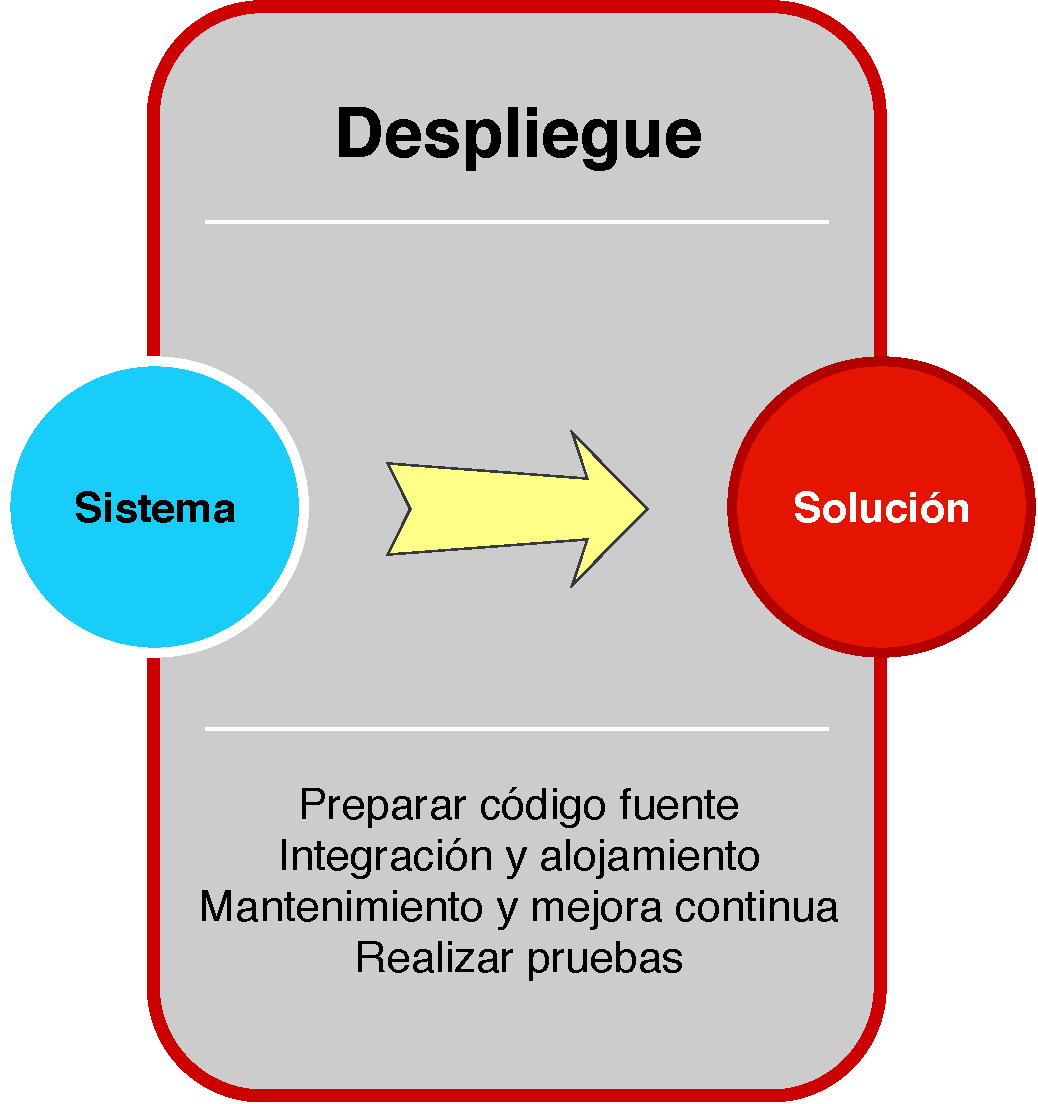
\includegraphics[width=0.5\textwidth]{capitulo_final/despliegue}
    \caption{Fase del despliegue}\label{fig:despliegue}
\end{figure}

La solución final deberá cumplir con todas las restricciones que fueron
desarrolladas a lo largo de la tesis, es decir, debe ser de uso fácil, mucha
exactitud y con funcionalidad dentro del laboratorio mismo.

Para concluir el proceso, se deben realizar pruebas del rendimiento del motor de
inferencia ya dentro de la Jetson Nano para asegurar que sea rápido y efectivo o
si no, optimizar más el modelo y medir la degradación en su rendimiento al ser
optimizado.

Debido a la falta de un microscopio para hacer pruebas de acoplamiento con el
adaptador impreso 3D y la cámara, estas quedan como trabajo a futuro. Hay que
probar si el adaptador efectivamente sirve para el propósito correcto, que no
filtra luz a la cámara y que esta se encuentra en la posición correcta para
capturar la luz que pasa por la laminilla.

La impresión de la carcasa final es un proceso sumamente tardado, en promedio se
tardará más de 3 días en la creación de todas las piezas que la componen. Sin
embargo, es un proceso necesario para el despliegue del sistema. Este proceso
también se requiere para poder realizar pruebas de ergonomía del uso del sistema
como un dispositivo discreto.

Ampliar las funciones de la interface para permitir al usuario tomar capturas de
células interesantes para compartirlas y gestionar conocimiento. Grabar video,
permitir la conexión de una pantalla externa más grande y distintos tipos de
pre-procesamiento de imagen para mejorar contrastes y nitidez también se
consideran parte del despliegue.

Para concluir el despliegue, es imperativo hacer pruebas con el usuario final,
es decir, el cito-tecnólogo. Para ello hay que crear un manual de usuario y
procedimientos para el correcto uso de la solución. Mucha retroalimentación con
el experto, un enfoque basado en \hyperlink{abbr}{UX} y una documentación clara
darán las herramientas necesarias para pulir la solución prototipo y convertirla
en un producto final.

Posteriormente se pretender crear un sistema central que controle todos los
dispositivos en uso. Que permita a los usuarios seleccionar y subir las imágenes
que el modelo haya clasificado mal para poder reentrenarlo y mejorar su
rendimiento dinámicamente. Las aplicaciones de \hyperlink{abbr}{DL} sufren de
una falta de datos correctamente etiquetados ya que se requieren bastantes y la
validación es cara y tardada, es por ello que crear una forma de auto-mejora de
la solución puede darle el empuje necesario para comportarse como se requiere
dentro de la vida real.